\documentclass[11pt]{article}
\newcommand{\oa}{\overline{a}}
\newcommand{\ob}{\overline{b}}
\newcommand{\oc}{\overline{c}}
\newcommand{\oi}{\overline{i}}

\newcommand{\integermodn}[1][n]{\Z/#1\Z}
\newcommand{\integermodnmul}[1][n]{(\Z/#1\Z)^{\times}}
\newcommand{\order}[1]{\left|#1\right|}
\newcommand{\modb}[1]{\left(mod \;\; #1 \right)}
\newcommand{\aut}[1]{Aut\left(#1\right)}
\newcommand{\actson}{\ensuremath{\curvearrowright}}

\newcommand{\heading}[1]{(#1)}
\newcommand{\bheading}[1]{\textbf{(#1)}}

% arg1=pdfurl arg2=pagenum arg3=text
\usepackage{url}
\usepackage{hyperref}
\hypersetup{colorlinks=true, linktoc=all, linkcolor=blue}
\newcommand{\linkbook}[3][../../abstract_algebra_dummit_and_foote.pdf]{
    \noindent\href[page=#2]{#1}{\urlstyle{rm}{#3}}
}

\usepackage[a4paper, total={6in, 8in}, margin=0.5in]{geometry}

\usepackage{listings}
\usepackage{hyperref}
\graphicspath{{assets/}}

\title{CSC446 A3}
\author{Peiqi Wang 1001132561}

\begin{document}
\maketitle


\section*{Problem 1} 
Implement Ritz-Galerkin method on equidistant grid with piecewise linear hat function for
\begin{align*}
    &-y'' + y = (\pi^2 + 1) \sin (\pi x) \quad x\in(0,1) \\
    &y(0) = 1\quad y'(1) = \frac{1}{2} (e-\frac{1}{e}) -\pi
\end{align*}
where the real solution to the problem is given by 
\[
    y(x) = \frac{1}{2} (e^x + e^{-x}) + \sin (\pi x)
\]
\begin{proof}[solution]
    Note this BVP is a special case of BVP that appeared in the textbook, so 
    \begin{align*}
        a_{k,l} 
        = \inner{\varphi_l'}{\varphi_k'} + \inner{\varphi_l}{\varphi_k}
        = \begin{cases}
            \frac{2(h^2+3)}{3h} & l=k \\
            \frac{h^2-6}{6h} & l = k-1,k+1 \\
            0 & \text{otherwise} \\
        \end{cases}
    \end{align*}
    for $k=1,2,\cdots, m-1$. Let 
    \[
        \varphi_0(x) = \p{\frac{1}{2} \p{e - \frac{1}{e}} - \pi} x  + 1
    \]
    satisfies the boundary conditions. Now we compute the right hand side of the linear system
    \begin{align*}
        b_k
        &= \inner{f}{\varphi_k} - a_{k,0} = \inner{f}{\varphi_k} - \inner{\varphi_0}{\varphi_k}\\
        &= \int_0^1 (\pi^2+1)\sin(\pi x) \varphi_k(x) dx 
            - \int_0^1 \varphi_0(x) \varphi_k(x) dx \\
        &= 
            \int_{(k-1)h}^{kh} (\pi^2 + 1) \sin(\pi x) \p{ 1-k+\frac{x}{h} } dx
            +\int_{kh}^{(k+1)h} (\pi^2+1) \sin(\pi x) \p{ 1+k-\frac{x}{h} } dx \\
        &\quad\quad -\int_{(k-1)h}^{kh} \p{\p{\frac{1}{2} \p{e - \frac{1}{e}} - \pi}x + 1} \p{ 1-k+\frac{x}{h}} dx \\
        &\quad\quad -\int_{kh}^{(k+1)h} \p{\p{\frac{1}{2} \p{e - \frac{1}{e}} - \pi}x + 1} \p{ 1+k-\frac{x}{h} } dx
    \end{align*}
    for $k=1,2,\cdots, m-1$. To allow for arbitrary approximate $y_m(x)$ at $x=1$, we have a basis function $\varphi_m(x)$ supported over $[x_{m-1}, x_m]$ only. The corresponding entries in $A$ and $b$ is as follows
    \begin{align*}
        a_{m, m-1} &= \frac{h^2-6}{6h} \\
        a_{m,m} &= \frac{h^2+3}{3h} \\
        b_m 
        &= \inner{f}{\varphi_k} - \p{
            -\inner{\varphi_0''}{\varphi_k} + \inner{\varphi_0}{\varphi_k}
        }  \\
        &=\int_{(m-1)h}^{mh} (\pi^2 + 1) \sin(\pi x) \p{ 1-m+\frac{x}{h} } dx\\
        &\quad \quad 
        -\int_{(m-1)h}^{mh}\p{\p{\frac{1}{2} \p{e - \frac{1}{e}} - \pi}x + 1} \p{ 1-m+\frac{x}{h}} dx
    \end{align*}
    Due to complexity of integrands that arises in the problem, we will numerically integrate all integrals with 5-point Gaussian Quadrature. Implementation is in \hyperref[q1code]{appendix}. We have maximum error as follows
    \begin{center}
        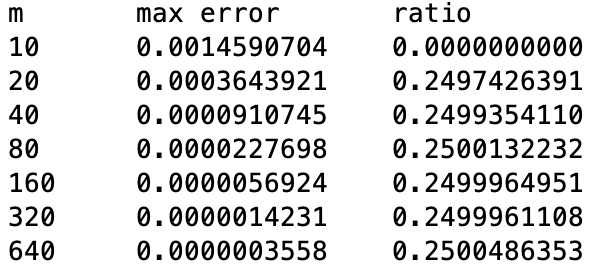
\includegraphics[width=3in]{q1_out}
    \end{center} 
    We see as $h=1/m$ halves, the maximum error decreases by a factor of 4.
\end{proof}


\section*{Problem 2} Repeat qestion 1, but use cubic B-spline basis instead of piecewise linear hat basis function. 

\begin{proof}[solution]
    Due to complexity of integrands that arises in the problem, we will numerically integrate all integrals with 5-point Gaussian Quadrature. We use the same $\varphi_0$ as previously described. Generic formula for $A$ and $b$ is given by 
    \begin{align*}
        a_{k,l} 
        &= \int_0^1 \pb{B_l'(x) B_k'(x) + B_l(x) B_k(x)} dx \\
        b_k 
        &= \int_0^1 \pb{f(x) B_k(x) + \varphi_0''(x)B_k(x) - \varphi_0(x) B_k(x)} dx
        = \int_0^1 \pb{f(x) B_k(x) - \varphi_0(x) B_k(x)} dx
    \end{align*}
    since $\varphi_0''(x)$ is a zero function on $[0,1]$. First derivates of $\varphi_k$ are computed from online integral calculator. Implementation is in \hyperref[q2code]{appendix}. Maximum error is given as follows
    \begin{center}
        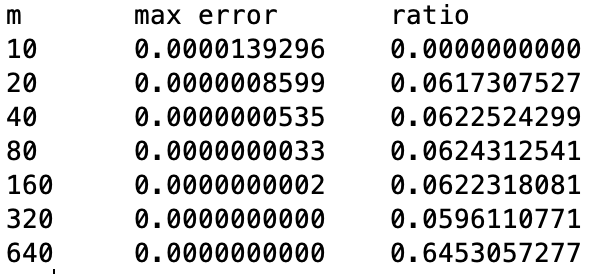
\includegraphics[width=3in]{q2_out} 
    \end{center}
    As $h$ halves, the maximum error decreases by a factor of 16. This expected for cubic basis functions, which makes erray decrease proportional to $h^4$. Compared to problem 1, where the linear hat basis function makes error decrease proportional to $h^2$, error for solution using B-spline basis decreases much faster.
\end{proof}



\section*{Problem 3} two-point bvp
\begin{align*}
    -y'' + 10^4 y &= 0 \quad \quad x\in(0,1) \\
    y(0) = y(1) = 1
\end{align*}
where real solution is 
\[
    y(x) = c_1 e^{100x} + c_2 e^{-100x}    
\]
where 
\[
    c_1 = \frac{1-e^{-100}}{e^100-e^{-100}}
    \quad 
    c_2 = \frac{e^100-1}{e^100-e^{-100}}
\]
\begin{proof}[solution]
    Use $\varphi_0(x) = 1$ and so $\varphi_0'(x) = 0$ for $x\in(0,1)$. We have
    \begin{align*}
        a_{k,l} 
            &= \inner{\varphi_l'}{\varphi_k'} + \inner{10^4\varphi_l}{\varphi_k} 
            = \int_0^1 \varphi_l'(x)\varphi_k'(x) + 10^4\varphi_l(x)\varphi_k(x) dx  \\
        b_k &= \inner{f}{\varphi_k} - a_{k,0} 
            = \inner{0}{\varphi_k} -\int_0^1 \varphi_0'(x)\varphi_k'(x) + 10^4 \varphi_0(x) \varphi_k(x) dx 
            = -10^4 \int_0^1 \varphi_k(x) dx
    \end{align*}
    where 
    \[
        \varphi_k'(x) = 
        \begin{cases}
            \frac{1}{x_k-x_{k-1}} & x\in [x_{k-1}, x_k] \\
            \frac{1}{x_k-x_{k+1}} & x\in [x_{k}, x_{k+1}] \\
            0 & \text{otherwise}
        \end{cases}
    \]
    We will numerically integrate all integrals with 5-point Gaussian Quadrature. We adapt new grid such that error over each element is approximately equal (\href{https://www.math.uci.edu/~chenlong/226/Ch4AFEM.pdf}{reference}). After plotting the real solution, we noticed that $y'$ has large magnitude near 0 and 1. So we choose a monitor function such that the adapted grid point is dense near 0 and 1. In particular, we used absolute value of the logit function 
    \[
        M(x) = \left| \log \frac{x}{1-x} \right|
    \]
    and constructed the grid as follows
    \begin{center}
        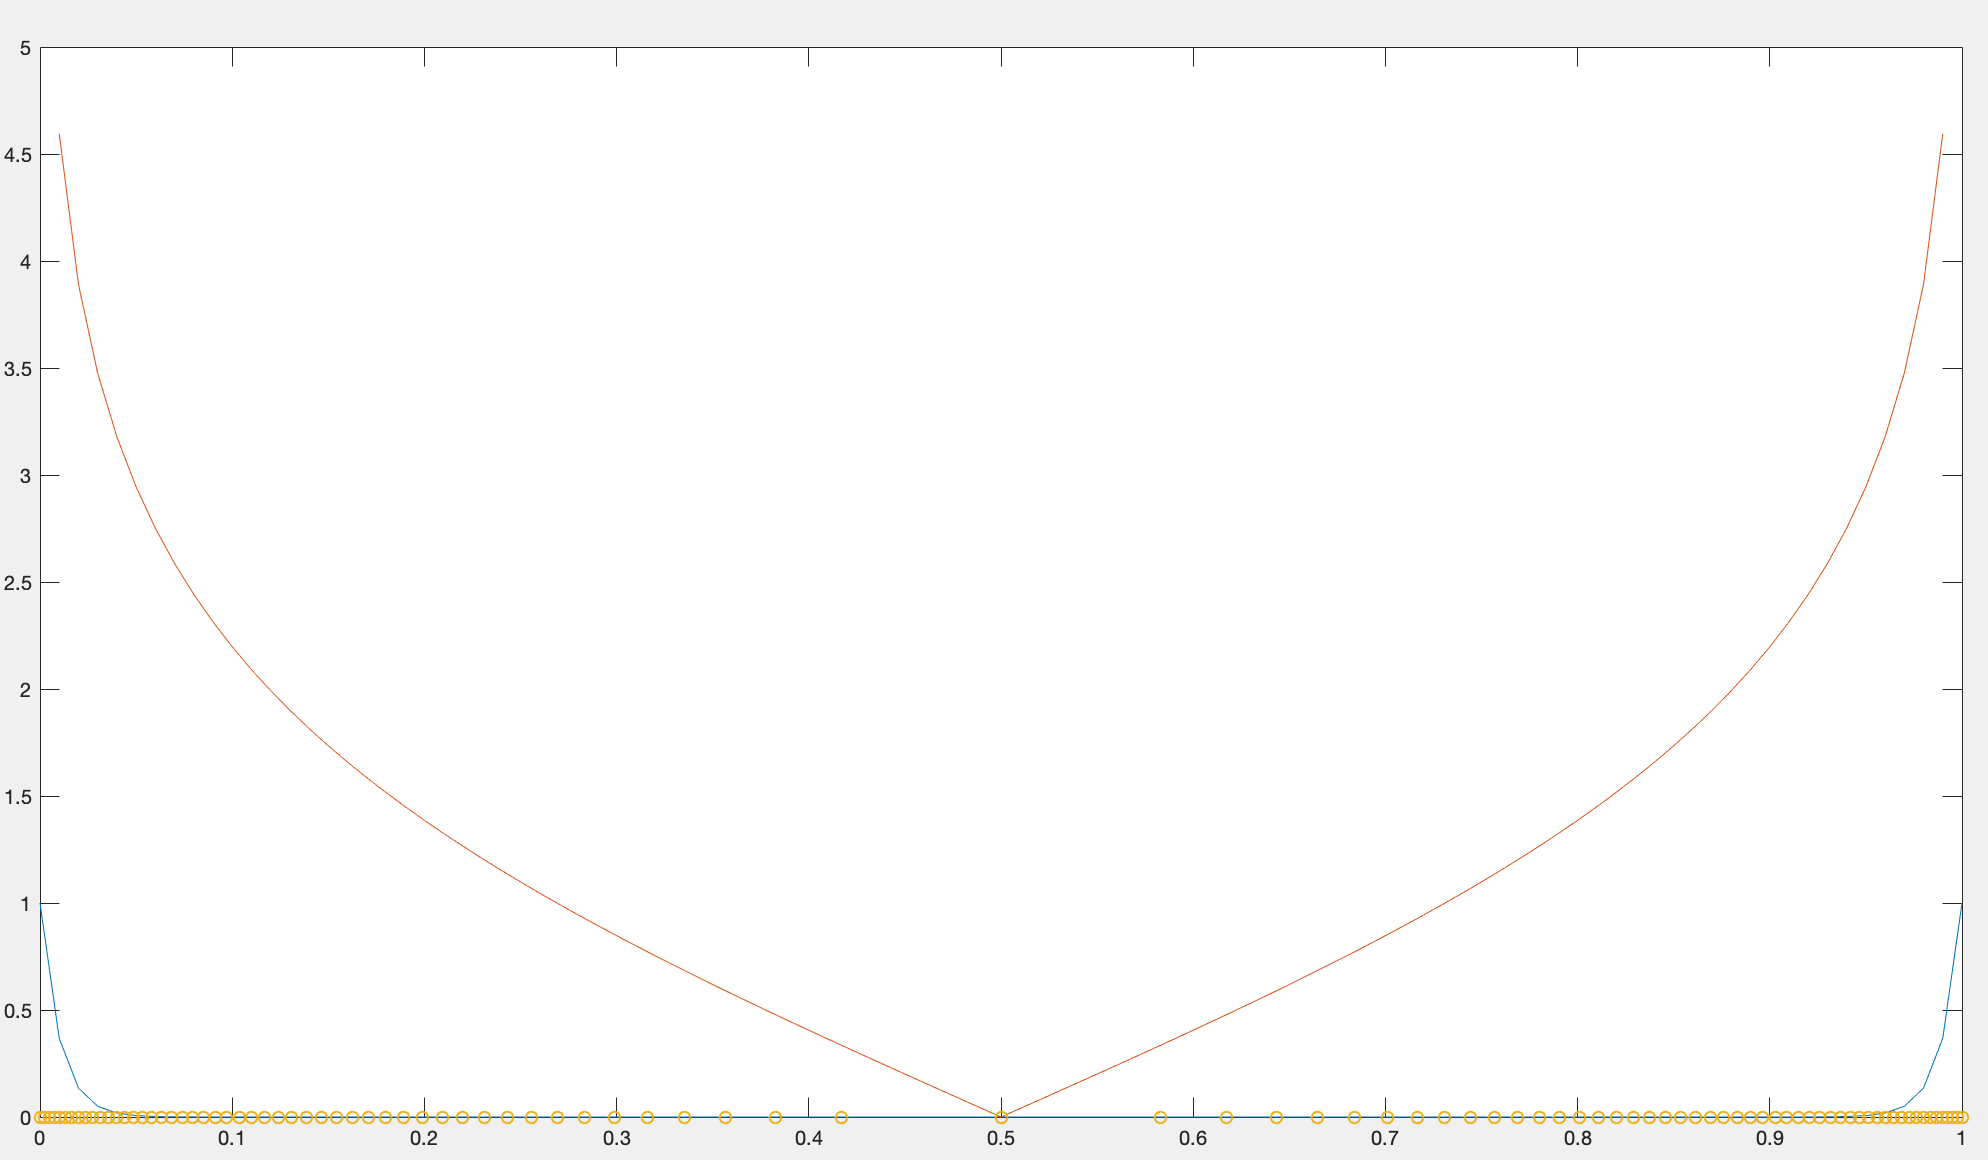
\includegraphics[width=\textwidth]{logit_matlab} 
    \end{center}
    Implementation is in \hyperref[q3code]{appendix}. We compare the maximum error using the equidistant (left) and adapted (right) grid.
    \begin{center}
        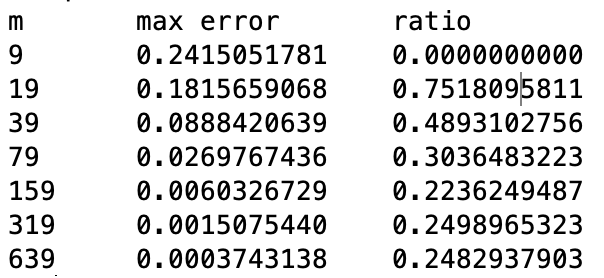
\includegraphics[width=3in]{q3_equidistant} 
        \quad\quad
        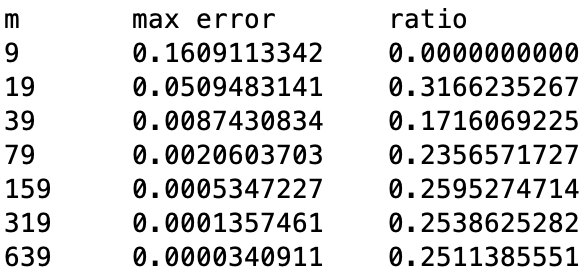
\includegraphics[width=3in]{q3_abslogit}
    \end{center}
    We noticed that, with the same number of basis functions, the maximum error on the adapted grid is at least an order of magnitude smaller to that of the equidistant grid.
\end{proof}

\section*{Problem 4}
2d bvp
\[
    -\nabla^2 u = -\frac{\partial^2 u}{\partial x^2} - \frac{\partial^2 u}{\partial y^2} = 32x(1-x) + 32y(1-y)
    \quad\quad
    x\in(0,1) 
    \quad 
    y\in(0,1)    
\]
with Dirichlet boundary, where the real solution is 
\[
    u(x,y) = 16x(1-x)y(1-y)    
\]
\begin{proof}[solution]
    Galerkin's equation for the above problem is derived in class, resulting in $m^2$ unknonwns. Note 
    \[
        \inner{\varphi_k}{\varphi_l} = 
        \begin{cases}
            \dfrac{2h}{3} & k = l \\
            \dfrac{h}{6} &  \abs{k-l} = 1\\
            0 & \text{otherwise}
        \end{cases}
        \quad\quad
        \inner{\varphi_k'}{\varphi_l'} = 
        \begin{cases}
             \dfrac{2}{h} & k = l \\
            -\dfrac{1}{h} &  \abs{k-l} = 1\\
            0 & \text{otherwise}
        \end{cases}
    \]
    \begin{align*}
        a_{(k,l),(i,j)} 
            &= \inner{\varphi_i'}{\varphi_k'}\inner{\varphi_j}{\varphi_l}
            + \inner{\varphi_i}{\varphi_k}\inner{\varphi_j'}{\varphi_l'}\\
            &= 
            \begin{cases}
                \dfrac{8}{3} & i = k \land j = l \\
                -\dfrac{1}{3} & \p{j=l \land \abs{i-k}=1}\lor\p{i=k \land \abs{j-l}=1} \\
                -\dfrac{1}{3} & \abs{k-i}=1 \land \abs{l-j}=1 \\
                0 & \text{otherwise}\\
            \end{cases} \\
        b_{(k,l)} 
            &= \inner{f}{\varphi_{k,l}} \\
            &= \int_0^1 \int_0^1 f(x,y) \varphi_{k,l}(x,y) dx dy \\
            &= \int_0^1 \int_0^1 (32x(1-x) + 32y(1-y))\varphi_k(x)\varphi_l(y) dx dy \\
            &= \int_0^1 \int_0^1 \pb{32x(1-x)\varphi_k(x)}\varphi_l(y)+\varphi_k(x) \pb{32y(1-y)\varphi_l(y)} dx dy \\
            &= \p{\int_0^1 32x(1-x)\varphi_k(x) dx} \p{\int_0^1 \varphi_l(y) dy} 
            +  \p{\int_0^1 \varphi_k(x) dx} \p{\int_0^1 32y(1-y)\varphi_l(y) dy}  \\
            &= h \p{\int_0^1 32x(1-x)\varphi_k(x) dx + \int_0^1 32y(1-y)\varphi_l(y) dy}
    \end{align*}
    for $k,l,i,j = 1,2,\cdots,m$. We can still use 5-point Gaussian Quadrature to integrate $b_{k,l}$ by using Fubini's theorem to simplify the expression of $b_{k,l}$ as shown above. Implementation is in \hyperref[q4code]{appendix}. Maximum error is given as follows
    \begin{center}
        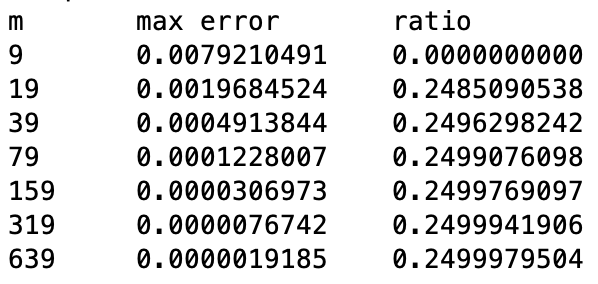
\includegraphics[width=3in]{q4_out} 
    \end{center}
    As $h$ halves, the maximum error decreases by a factor of 4. 
\end{proof}


\newpage
\section*{Appendix}
\lstinputlisting[language=matlab]{code/gq.m}
\newpage
\section*{Problem 1 code}
\label{q1code}
\lstinputlisting[language=matlab]{code/q1.m}
\newpage
\section*{Problem 2 code}
\label{q2code}
\lstinputlisting[language=matlab]{code/q2.m}
\newpage
\section*{Problem 3 code}
\label{q3code}
\lstinputlisting[language=matlab]{code/q3.m}
\newpage
\section*{Problem 4 code}
\label{q4code}
\lstinputlisting[language=matlab]{code/q4.m}


\end{document}